\documentclass[
  journal=pasa,
  manuscript=review, %% or "review"
  year=2021,
  volume=37,
]{cup-journal}

\usepackage{microtype,siunitx,booktabs}
\usepackage{natbib}
\usepackage{tabularx}
\usepackage{longtable}
\usepackage{xcolor}
\definecolor{darkblue}{RGB}{0,32,135}
\sisetup{detect-all,separate-uncertainty=true}
%------------------VISITADOR-------------------------------------------------

\title{Aplicación de ciencia de datos en metodologías para el diagnóstico del cáncer de mama}

\author{Jorge Armando Millán Gómez, Lilia Edith Aparicio Pico}
\affiliation{Grupo de Investigación en Telemedicina, Universidad Distrital "Francisco José de Caldas", Facultad de Ingeniería, Bogotá,Colombia}
\email[J. A. Millán ,L. E. Aparicio]{jamillang@correo.udistrital.edu.co, eaparicio@udistrital.edu.co}

%\author{M. Sokolowski}
%\affiliation{International Centre for Radio Astronomy Research, Curtin University, Bentley, WA6102, Australia}
% \alsoaffiliation{Joint first authors}

%\author{R. Wayth}
%\affiliation{International Centre for Radio Astronomy Research, Curtin University, Bentley, WA6102, Australia}

%\author{D. Ung}
%\affiliation{International Centre for Radio Astronomy Research, Curtin University, Bentley, WA6102, Australia}

%\handlingeditor{Excellent E Editor}

\doi{10.1017/pasa.2022.32}

\received {20 03 2022}
\revised  {20 03 2022}
\accepted {20 03 2022}
\published{19 Abril 2022}

%\keywords{metodología, ciencia de datos, cáncer de mama, diagnostico.}
 %% First letter not capped
% \jel{Q11; Q12; D81; M31}
% \msc{Q14; Q18; E21}
% \abbreviations{
%     BDHS: Bangladesh Demographic and Health Survey, 
%     IDA: Fe-deficiency anaemia, 
%     IFA: Fe-folic acid, 
%     MNP: multiple micronutrient powder, 
%     VAD: vitamin A deficiency
% }
\begin{document}

\section*{Introducción}
El Cáncer de mama ocupa el primer lugar con mayor número de muertes en Colombia ocupando el primer puesto en la tasa de letalidad sobre los demás tipos de cáncer afectando a mujeres de todas las edades. En el año 2020 los casos detectados de cáncer de mama en Colombia fueron 15.509 de los cuales 4.411 terminaron en muerte\cite{InternationalAgencyforResearchonCancer2020}. Este tipo de cáncer se origina cuando las células mamarias comienzan a crecer sin control convirtiéndose en células malignas que normalmente forman un tumor que a menudo se puede observar en una radiografía o se puede palpar como una masa o bulto\cite{Sauer2019}. El pronóstico anticipado de esta enfermedad se ha convertido en una necesidad de investigación debido a que puede facilitar el tratamiento preventivo para evitar su letalidad en un estado avanzado. Muchos investigadores han puesto sus esfuerzos en los diagnósticos y pronósticos del cáncer de mama, cada técnica tiene una tasa de precisión diferente que varía según las diferentes situaciones, herramientas y conjuntos de datos que se utilizan. En la actualidad la ciencia de datos es utilizada por diferentes investigadores para modelar la progresión y el tratamiento de afecciones cancerosas debido a su capacidad para detectar características significativas en conjuntos de datos complejos. La medicina basada en datos tiene la capacidad no solo de mejorar la velocidad y precisión del diagnóstico de enfermedades genéticas, sino también de desbloquear la posibilidad de tratamientos médicos personalizados\cite{Baker2018}. Una parte fundamental de la ciencia de datos es el uso de algoritmos de ML\footnote{Machine Learning} y DL\footnote{Deep Learning} los cuales se componen de tres estrategias principales que consisten en preprocesamiento, extracción de características y clasificación. La extracción de características es fundamental en el diagnóstico del cáncer de mama ya que ayuda a identificar datos relevantes en una categoría maligna o benigna\cite{Fatima2020}. Adicionalmente, en los últimos años, el aumento de la potencia de las computadoras, junto con los avances matemáticos, ha permitido el uso de las redes neuronales complejas de múltiples capas (profundas) las cuales han mejorado el rendimiento de la interpretación automática de imágenes oncológicas altamente estandarizadas\cite{Mann2020}.

En otra instancia la literatura muestra que la mayoría de los casos de estudio de investigación científica y de desarrollo de aplicaciones se han dado sobre la aplicación de estas diferentes técnicas a imágenes médicas. Asimismo, otra forma de obtener información relevante es a través de técnicas de detección por Biopsia como es el caso de la aspiración por aguja Fina (FNA\footnote{Fine Needle Aspiration}) y aspiración por aguja gruesa (CNB\footnote{Core Needle Biopsy}) y las técnicas basadas en el análisis de receptores de estrógeno en datos metabolómicos. 
\\\\
Esta investigación se va centrar esencialmente en diseñar una metodología aplicada a técnicas en ciencias de datos partiendo del análisis de un data-set conformado por dicha información para poder comprobar la efectividad de estos métodos médicos en la detección y el diagnóstico del cáncer de mama, lo que nos permitirá evaluar la validez de tener imágenes diagnosticas u otros tipos de datos oncológicos. Esto va a repercutir, en la facilidad de la obtención de los datos y el procesamiento de la información para el diagnóstico y pronostico del padecimiento de esta enfermedad.

\section{Detección y diagnóstico del cáncer de mama}

El cáncer de mama, con su causa incierta, ha capturado la atención de los cirujanos en todas las épocas. A pesar de siglos de laberintos teóricos y preguntas científicas, el cáncer de mama aún es una de las enfermedades humanas más temibles \citep{Bland2009}. Segun \citep{Fatima2020}, el cáncer de mama se origina a través de tumores malignos, cuando el crecimiento de la célula se descontrola provocando que muchos tejidos grasos y fibrosos de la mama inicien un crecimiento anormal, lo cual tiene como consecuencia que las células cancerosas se diseminen por los tumores causando las diferentes etapas del cáncer. \citep{Fatima2020} exponen que existen diferentes tipos de cáncer de mama \citep{Sun2017}, que se producen cuando las células afectadas y tejidos diseminados se esparcen por todo el cuerpo. Pongamos por caso, el primer tipo de cáncer denominado \textit{Carcinoma ductal in situ (DCIS)} el cual es un tipo de cáncer no invasivo \citep{Hou2020}, que se produce cuando las células anormales se propagan fuera de la mama. El segundo tipo de cáncer es el \textit{Carcinoma ductal invasivo (IDC)}, también conocido como carcinoma ductal infiltrante \citep{Chaudhury2011}. Este tipo de cáncer ocurre cuando las células anormales de la mama se diseminan por todos los tejidos mamarios. Generalmente este tipo de cáncer se encuentra en los hombres \citep{Page1982}. El tercer tipo de cáncer es el cáncer de \textit{Tumores mixtos (MTBC)} también conocido como cáncer de mama invasivo \citep{Tuck1997} causado por las células anormales de los conductos y las células lobulillares \citep{Lee2017}. El cuarto tipo de cáncer es el cáncer de mama \textit{Lobulillar (LBC)} \citep{Masciari2007} que ocurre dentro del lóbulo y aumenta las posibilidades de otros cánceres invasivos. El quinto tipo cáncer es el cáncer de mama \textit{mucinoso (MBC)} o de \textit{mama coloide} \citep{Memis2000} que ocurre debido a las células ductales invasivas cuando los tejidos anormales se extienden alrededor del conducto \citep{Gradilone2011}. El sexto y ultimo tipo de cáncer es el cáncer de mama \textit{inflamatorio (IBC)}, el cual causa hinchazón y enrojecimiento del pecho. Este tipo de cáncer de mama es de rápido crecimiento, y comienza a aparecer cuando los vasos linfáticos se obstruyen en células rotas \citep{Robertson2010}.

Según \citep{Brunicardi2010}, en la mayoría de casos detectados la mujer descubre una tumoración en su mama. Otros signos y síntomas que se presentan menos a menudo comprenden: crecimiento o asimetría de la mama, alteraciones y retracción del pezón o telorrea, ulceración o eritema de la piel de la mama, una masa axilar y molestia musculoesquelética. Case señalar, que si se detectan alguno de los síntomas anteriores este tipo de cáncer puede ser detectado por medio de los procedimientos basados en \textit{Exploración Física}, \textit{Técnicas de imagen} y \textit{Biopsias}. 

A nivel de \textit{Exploración física}, el cáncer de mama puede ser detectado por el oncólogo por medio de los métodos de \textit{Inspección} y \textit{Palpación}. Con estos métodos, se registran la simetría, el tamaño y la forma de la mama, así como cualquier evidencia de edema (piel de naranja), retracción del pezón o de la piel y eritema \citep{Brunicardi2010}.

En la actualidad, muchas \textit{Técnicas de imagen} se utilizan ampliamente para proporcionar un diagnóstico preciso de las lesiones mamarias\citep{Tamam2021}, entre estas técnicas las mas relevantes son las siguientes: \textit{La Mamografía} que hace uso de una unidad mamográfica que consta de un tubo de rayos X que encapsula un cátodo y un ánodo. La mama se coloca sobre el detector y se comprime mediante un dispositivo de placas paralelas, el cual mantiene la mama inmóvil y evita el desenfoque por movimiento, esto con el propósito de reducir el grosor del tejido que deben atravesar los rayos x \citep{Ebrahimi2019}; \textit{La ductografía} que identifica de lesiones en pacientes con secreción del pezón. Este método es eficaz para localizar e identificar las lesiones intraductales por medio de un examen mamográfico realizado tras el llenado retrógrado de los conductos galactóforos con material de contraste \citep{Hirose2007}; \textit{La Ecografía} que permite obtener imágenes de alta resolución por medio de un pequeño transductor (sonda) de alta frecuencia que envía ondas sonoras inaudibles al interior de la mama y recibe el eco de las ondas procedentes de los órganos internos, los fluidos y los tejidos \citep{Hasan2019}; y \textit{La Resonancia Magnética (MRI\footnote{Magnetic Resonance Imaging}) }que es utilizada cuando las lesiones en la mama no se pueden evaluar fácilmente mediante otras técnicas. Para lograrlo, utiliza bobinas receptoras de radiofrecuencia (RF) para detectar una señal emitida por los tejidos tras la excitación de un campo electromagnético que obliga a los protones alinearse a la anatomía de la zona de interés en tamaño y forma \citep{Tse2014}.

Hay que mencionar, además que actualmente existen dos modalidades para obtener un diagnóstico por \textit{Biopsia} para un paciente que presenta una anomalía mamaria. Por un lado tenemos, la biopsia para mamas con \textit{lesiones palbables} tambien denominada \textit{percutánea} o \textit{mínimamente invasiva}. Estas biopsias incluyen la aspiración con aguja fina (FNA) y con con aguja gruesa (CNB). Las biopsias quirúrgicas abiertas se denominan a veces biopsias por escisión o biopsias por incisión. La biopsia por \textit {escisión} indica la extirpación completa de la lesión, mientras que la biopsia por \textit {incisión} indica la extirpación de parte de la lesión \citep{Greenfield2012}. En el caso de las \textit{lesiones no palpables}, las modalidades de imagen como la ecografía (US), la mamografía y la resonancia magnética (MRI) son complementos útiles para identificar y localizar la lesión de interés. La decisión de cuándo realizar una biopsia de mama depende de los antecedentes del paciente, los hallazgos de la exploración física y las imágenes radiológicas. El objetivo principal de la biopsia es obtener un diagnóstico tisular que pueda ayudar a dictar el tratamiento y la planificación preoperatoria, si está indicado. Por lo tanto, es imprescindible elegir una técnica de biopsia que optimice las posibilidades de obtener un diagnóstico preciso y que, al mismo tiempo, minimice los costes, limite las molestias del paciente y reduzca la necesidad de repetir el procedimiento \citep{Samilia2018} .
	
\section{Aplicaciones del ML y DL en el diagnostico del cáncer de mama}
 Diversas técnicas de ML y DL aplicadas en el diagnóstico del cáncer de mama han sido propuestas por una gran cantidad de investigadores. Aunque para el cribado de información se excluyeron los estudios que tienen un enfoque en técnicas y no en metodologías de ciencia de datos, se seleccionaron las siguientes investigaciones por su relevancia y aporte para el diagnostico del cáncer de mama debido a que brindan una gran cantidad de información y son un punto de partida importante para aplicar la ciencia de datos con dicho fin. Las investigaciones seleccionadas como referentes a nivel de técnicas se muestran a continuación:

\citep{Alakwaa2018} realizaron la identificación de subtipos moleculares sobre datos metabolómicos por medio de algoritmos de DL y ML para determinar el pronóstico del cáncer de mama y la selección terapéutica. Para ello, la investigación se basa en la clasificación de dicho cáncer en cuatro subtipos moleculares: Luminal A ($ER +, PR \pm$ y $HER2-$), Luminal B ($ER +, PR \pm,$ y $HER2\pm$), $HER2-$ enriquecido ($ER-, PR-$ y $HER2 +$) y triple negativo ($ER-, PR-$ y $HER2 -$). Estos subtipos son generados a partir de las proteínas de factor de crecimiento epidérmico receptor 2 (HER2), receptor de progesterona (PR) y receptor de estrógeno (ER) encargadas de estimular el crecimiento y la diferenciación celular. Los resultados de supervivencia difieren significativamente entre estos subtipos. Los subtipos luminales A y B tienen un pronóstico benigno sin embargo, los tumores triple negativos y los tumores $HER2$ tienen un pronóstico maligno. Para la investigación se utilizó un data-set conformado por 271 muestras de cáncer de mama ($204$ $ER+ $ y $67$ $ER- $) del Departamento de Patología del Hospital Charité. Posterior a eso para complementar dicho data-set se midieron un total de 162 metabolitos con estructura química conocida mediante cromatografía de gases para todas las muestras de tejido. Para realizar la clasificación de los datos metabólicos obtenidos se utilizó una Red Neuronal FNN\footnote{Feedforward Neural Network} y los siguientes modelos de ML: RF, SVM, RPART\footnote{Recursive Partitioning}, LDA\footnote{Linear Discriminant Analysis}, PAM\footnote{Microarray Prediction Analysis} y GBM\footnote{Gradient Boosting Machine}. Posteriormente, se realizó una validación cruzada (Cross-validation) con el 80\% de los datos de entrenamiento y se probaron los modelos con el 20\% de los datos restantes. Para finalizar, se utilizaron las medidas AUC\footnote{Area Down The Curve} y ROC\footnote{Receiver Operating Characteristic Curve} para evaluar el rendimiento general de los dichos modelos. En conclusión, esta investigación determino que las FNN muestran una precisión de predicción (AUC = $0,93$) mayor sobre los métodos de ML al realizar la clasificación del cáncer de mama en los subtipos moleculares basados en el receptor de estrógeno(ER).

\citep{Nateghi2021} proponen de un sistema basado en métodos de DL y ML para la predicción de la proliferación tumoral a partir de imágenes WSI \footnote{ Whole Slide Images } obtenidas del recuento mitótico. La proliferación tumoral, que se correlaciona con el grado del tumor, es un biomarcador crucial que indica el pronóstico de las pacientes con cáncer de mama. El método más utilizado para predecir la velocidad de proliferación tumoral es el recuento de figuras mitóticas en los portaobjetos histológicos de hematoxilina y eosina ($H\&E$). El recuento manual de mitosis consiste en identificar células tumorales implicadas en el proceso anormal de la división celular. Para la investigación se utilizó el data-set proporcionado por el desafío de evaluación de la proliferación tumoral (TUPAC16) en donde el objetivo es evaluar algoritmos que predicen las puntuaciones de proliferación tumoral a partir de imágenes WSI. Primero, al considerar el tejido epitelial como regiones de actividad de mitosis, los investigadores propusieron un método de detección de regiones de interés basado en DL para seleccionar las regiones de alta actividad de mitosis a partir de las imágenes proporcionadas en el desafío. Posteriormente, se entrenó un conjunto de redes neuronales para detectar la propagación de la mitosis en distintas áreas seleccionadas. Para finalizar, los investigadores entrenaron el modelo SVM para predecir la puntuación final de proliferación tumoral. La precisión del algoritmo entrenado logró una medida-F del 73,81\% y un coeficiente kappa ponderado de 0,612, respectivamente, superando significativamente otros algoritmos que participaron en el desafío TUPAC16. Como conclusión de la investigación, los resultados experimentales demuestran que el algoritmo propuesto basado en el paradigma de DL y ML mejoró considerablemente la precisión de la predicción de la proliferación tumoral y proporciono un modelo con una precisión confiable para respaldar la toma de decisiones a nivel médico.

\citep{McKinney2020} desarrollaron un modelo de DL para identificar el padecimiento del cáncer de mama mediante imágenes mamográficas obtenidas en el Reino Unido y EE. UU. La mamografía tiene como objetivo identificar el cáncer de mama en las primeras etapas de la enfermedad, cuando el tratamiento puede tener más éxito. A pesar de la existencia de diversas técnicas de detección del cancér de mama en todo el mundo, la interpretación de las mamografías se ve afectada por altas tasas de falsos positivos y falsos negativos. El data-set del Reino Unido consistió en mamografías recopiladas de 25,856 mujeres entre 2012 y 2015 en dos centros médicos en Inglaterra, donde las mujeres se examinan cada tres años. Incluyó a 785 mujeres a las que se les realizó una biopsia y a 414 mujeres con una diagnóstico maligno del cáncer dentro de los 39 meses posteriores a la obtención de imágenes. El data-set de EE. UU consistió en mamografías que se recolectaron entre 2001 y 2018 de 3.097 mujeres en un centro médico académico. Se incluyeron imágenes de las 1511 mujeres a las que se les realizó una biopsia durante este período de tiempo y de un subconjunto aleatorio de mujeres que nunca se sometieron a una biopsia. Entre las mujeres que recibieron una biopsia, 686 fueron diagnosticadas con cáncer dentro de los 27 meses posteriores a la obtención de las imágenes. Los casos que fueron diagnosticados como positivos para cáncer fueron acompañados de un diagnóstico confirmado por biopsia dentro del período de seguimiento. una reducción absoluta del 5,7\% y 1,2\% (EE.UU. Y Reino Unido) en falsos positivos y del 9,4\% y 2,7\% en falsos negativos. En la investigación los data-set obtenidos no se utilizaron para entrenar ni ajustar el modelo basado IA. Como resultados, la investigación proporciono evidencia de la capacidad del modelo basado en IA y DL para generalizarse desde el Reino Unido a los EE.UU. En un estudio independiente de seis radiólogos, el sistema de IA superó el diagnóstico obtenido por dichos radiólogos con una precisión (AUC-ROC) mayor que la generada por el radiólogo promedio. Además, para comprobar la predicción del modelo los investigadores realizaron una simulación en la que el sistema de IA participó en el proceso de doble lectura de diagnóstico que se utiliza en el Reino Unido y se descubrió que el sistema de IA mantuvo un rendimiento elevado y redujo la carga de trabajo del segundo lector en un 88\%. Como conclusión, esta investigación demostró que las técnicas de IA mejoran la precisión y la eficiencia de las técnicas tradicionales para la detección del cáncer de mama.


\citep{Mullooly2019} utilizaron técnicas de DL para identificar correlaciones histológicas en biopsias de la densidad mamaria obtenidas por técnicas radiológicas para determinar el cáncer de mama entre mujeres con una densidad del tejido fibroglandular alto o bajo. La densidad de la mama es una característica radiológica que refleja el contenido de tejido fibroglandular en relación con el área o el volumen de la mama y es considerada como un factor de riesgo de padecer cáncer. En la investigación se evaluaron imágenes digitalizadas teñidas con hematoxilina y eosina ($H\&E$) de biopsias de 852 pacientes. La densidad mamaria se evaluó como volumen fibroglandular global y localizado. Posteriormente, los investigadores modelaron una Red Neuronal CNN para caracterizar la composición de $H\&E$. En total, se extrajeron 37 características de la salida de la red, que describen las cantidades de tejido y la estructura morfológica. Se entrenó un modelo de regresión por Bosque Aleatorio (RF) para identificar correlaciones predictivas del volumen fibroglandular en 588 pacientes. Se evaluaron las correlaciones entre el volumen fibroglandular predicho y cuantificado radiológicamente en 264 pacientes independientes. Se entrenó un segundo clasificador de bosque aleatorio (RF) para predecir el diagnóstico invasivo vs. el diagnóstico benigno; el rendimiento de los algoritmos se evaluó utilizando el área bajo la curva (AUC). Utilizando características extraídas, los modelos de regresión predijeron el volumen fibroglandular global con una precisión de 0,94 y localizado con una precisión de 0,93 teniendo como base el contenido del estroma graso y no graso representando las correlaciones más fuertes seguidas de la cantidad de tejido epitelial. Para predecir el cáncer entre el volumen fibroglandular elevado y bajo, el clasificador logró un valor AUC de 0,92 y 0,84, respectivamente, siendo las características de tejido epitelial las más importantes. Estos resultados sugieren que el estroma no graso, la cantidad de tejido graso y el tejido epitelial predicen el volumen fibroglandular. Como conclusión, la investigación demostró que los modelos de DL y ML permiten identificar correlaciones histológicas con riesgo de cáncer en pacientes con alta y baja densidad de tejido fibroglandular.

\citep{Hu2020} desarrollaron una técnica para el diagnóstico asistido por computadora CAD\footnote{Computer-Aided Diagnosis} bajo el paradigma de aprendizaje por transferencia profunda para realizar la diagnosis del cáncer de mama utilizando mpMRI\footnote{Multiparametric Magnetic Resonance Imaging}.El estudio incluyó imágenes clínicas de resonancia magnética de 927 lesiones únicas de 616 mujeres, en donde se excluyeron las imágenes de lesiones que no presentaban una lesión visible, lesiones que no tenían validación de diagnóstico final, o lesiones que no pudieron ser claramente asignadas en a la categoría benigna ni maligna. Cada estudio de resonancia magnética RM\footnote{Magnetic Resonance}, incluyó una secuencia con contraste dinámico DCE\footnote{Dynamic Contrast-Enhanced} y una imagen de RM ponderada en un radio T2w\footnote{T2 weighted image}. Se utilizó una Red Neuronal CNN previamente entrenada para extraer características de las imágenes DCE y T2w, y se entrenaron modelos SVM en las características de CNN para distinguir entre lesiones benignas y malignas. La información de las imágenes de resonancia magnética con contraste dinámico (DCE) y ponderada en T2w se añadió al modelo IA de tres formas diferentes: fusión de imágenes, fusión de características y fusión de clasificadores. La fusión de imágenes, se utilizó para crear una imagen compuesta RGB con base a las imágenes DCE y T2w. La fusión de características, para combinar las características generadas por las redes neuronales convolucionales con base a las imágenes DCE y T2w para posteriormente ser utilizadas como entrada en un algoritmo de máquina de vectores de soporte (SVM). La fusión clasificadora se utilizó para calcular la probabilidad de malignidad por medio de voto suave (soft-voting) con base al resultado obtenido por el algoritmo SVM al analizar las imágenes DCE y T2w. El rendimiento de los modelos de DL se evaluó utilizando la curva (ROC) y fue comparado utilizando la prueba DeLong. El método de fusión de características superó estadísticamente de manera significativa a los demás métodos. En conclusión, el método propuesto de aprendizaje de transferencia profunda CAD para mpMRI pudo mejorar el diagnóstico del cáncer de mama al reducir la tasa de falsos positivos y mejorar el valor predictivo positivo en la interpretación de imágenes obtenidas por resonancia magnética.

\citep{Shia2021}, propusieron  un método de ML y diseño de una metodología para el análisis de la clasificación de tumores de mama benignos y malignos en imágenes de ultrasonido sin necesidad de un procesamiento de selección regional tumoral a priori.  Las imágenes se recopilaron desde el 1 de enero de 2017 hasta el 31 de diciembre de 2018. En total, se examinaron 370 masas benignas y 418 malignas, y se estudiaron a 677 pacientes en este estudio. Los criterios de exclusión para pacientes con tumores benignos incluyeron tipos de tejido que se asociaron con las siguientes afecciones: inflamación (incluida la autoinflamación, inflamación crónica e inflamación xantogranulomatosa), abscesos y dermatitis espongiótica. Para los pacientes con tumores malignos, los criterios de exclusión incluyeron casos con tipos de tejido incompletos, clasificación de categoría BI-RADS\footnote{Breast Imaging Reporting and Data System} desconocida o informes de imágenes incompletas. Las edades de los pacientes oscilaron entre los 35 y los 75 años.  El data-set recopilado constaba de 677 imágenes (Benignas: 312, maligno: 365) obtenidas de diferentes centros oncológicos de Estados Unidos. Una vez generado el data-set de estudio se procedió a realizar la extracción de características de las imágenes a través del método de histograma de gradientes orientados HOG\footnote{Histogram of Oriente Gradients} y el método histograma piramidal de gradientes orientados PHOG\footnote{Pyramid Histogram of Orientad Gradients}. Adicionalmente, se utilizó el método FAST\footnote{Features from the Accelerated Segment Test} para determinar si se podían extraer características de clasificación importantes de las imágenes preliminares. El HOG se utilizó para extraer información útil y descartar información redundante para simplificar la clasificación de imágenes calculando y contando histogramas de gradiente de áreas específicas. La distancia entre dos descriptores de imágenes PHOG refleja la medida en que las imágenes contienen formas similares y corresponde a sus diseños espaciales y el método FAST permite un rendimiento mayor que otros métodos en la detección de esquinas de los mamogramas para extraer puntos característicos y luego rastrear y mapear objetos con características relevantes en dichas imágenes. El siguiente paso fue realizar la selección de características por medio de la técnica de selección de características basada en correlación CFS\footnote{Correlation Based Feature Selection} para evaluar los atributos importantes, y crear un subconjunto de datos considerando las habilidades predictivas junto con el grado de redundancia. La función de evaluación se utilizó para evaluar subconjuntos que contenían características que estaban altamente correlacionadas con la clase y no estaban correlacionadas entre sí. Se ignoraron las características irrelevantes y se excluyeron las características redundantes. Finalmente, se realizó la clasificación de características con base en la combinación de aprendizaje ponderado localmente LWL\footnote{Local Weighted Learning }, la optimización secuencial mínima SMO\footnote{Sequential Minimal Optimization} y el  método KNN.  Para la evaluación del desempeño de la clasificación, se utilizó la técnica de validación cruzada para determinar el porcentaje de error, la media, la desviación estándar y el intervalo de confianza para los algoritmos de referencia.  La precisión diagnóstica se estimó comparando las curvas AUC y ROC con la prueba no paramétrica de DeLong. El rendimiento de clasificación del conjunto de datos de imágenes mostró una sensibilidad del 81,64\% y una especificidad del 87,76\% para imágenes malignas con AUC de 0,847. Los valores predictivos positivos y negativos fueron 84,1 y 85,8\%, respectivamente. En conclusión, la comparación de los diagnósticos médicos y el diagnóstico generado por el modelo de ML propuesto arrojó resultados similares. Esto indica la posible aplicabilidad del ML en la generación de diagnósticos clínicos.

\citep{Shen2019} desarrollaron un algoritmo de DL que puede detectar con precisión el cáncer de mama en mamografías usando un entrenamiento e2e \footnote{end-to-end} que aprovecha de manera eficiente los data-sets de imágenes mamográficas obtenidas a través de diagnósticos asistidos por ordenador CAD . En este enfoque las anotaciones para identificación de lesiones en la mama obtenidas de las imágenes mamográficas solo se utilizaron en la etapa de entrenamiento inicial, y las etapas posteriores requirieron solo las características obtenidas a nivel de imagen, eliminando la dependencia de diagnósticos obtenidos de estas anotaciones. El algoritmo generado fue testeado con dos data-set de prueba. El primer data-set fue obtenido de la base de datos de mamografías digitales del sitio web CBIS-DDSM. Este data-set almacenaba 2478 imágenes de mamografías de 1249 mujeres e incluía vistas tanto craneocaudales (CC) como oblicuas mediolaterales (MLO), además contaba con etiquetas confirmadas patológicamente en una categoría benigna o maligna para la mayoría de los exámenes. Con este data-set, el modelo logró una predicción con un valor AUC de 0,88 y el promedio de cuatro modelos entrenados posteriormente mejoró esta predicción a valor AUC de 0,91 con una sensibilidad de 86,1\% y especificidad de 80,1\%. El segundo data-set fue obtenido de la base de datos de mamografías digitales INbreast FFDM\footnote{Full-Field Digital Mammography} la cual contenía información de 115 pacientes y 410 mamografías, este data-set también incluía vistas CC y MLO. Con el segundo data-set el modelo logró una predicción con valor AUC de 0,95, y el promedio de cuatro modelos entrenados mejoró el AUC a 0,98 con una sensibilidad de 86,7\% y especificidad de 96,1\%. La investigación demostró que el entrenamiento generado en una Red Neuronal CCN con el enfoque e2e CBIS-DDSM se puede transferir a imágenes FFDM de INbreast utilizando solo un subconjunto de datos para ajustar el modelo y sin depender de la disponibilidad de anotaciones de lesiones. Estos hallazgos demostraron que los métodos de DL se pueden utilizar para lograr una alta precisión de diagnosis en mamografía heterogéneas y es muy prometedor para mejorar las herramientas clínicas para reducir la detección de falsos positivos y falsos negativos de cáncer de mama.

\citep{Naik2020} utilizaron el paradigma de DL con base al diagnóstico del cáncer de mama a partir del estado molecular del receptor de Estrógeno ERS\footnote{Estrogen Receptor Status},determinado por los patólogos a partir de la tinción inmunohistoquímica IHC\footnote{Inspection Immunohistochemistry} que destaca la presencia de antígenos de superficie celular del tejido obtenido a través de una biopsia. Para lograrlo, se recopilaron imágenes WSI teñidas con hematoxilina y eosina (H\&E) del data-set obtenido del Banco Australiano de tejidos para el cáncer de mama ABCTB\footnote{Australian Breast cáncer Tissue Bank}, que contenía 2535 imágenes de exámenes realizados  a pacientes y el data-set obtenido del Atlas genómico del cáncer TCGA\footnote{The Cancer Genomic Atlas}, que contenía 1014 imágenes de 939 pacientes. Ambos conjuntos de datos informaban el estado de la presencia de receptor de Estrógeno (ER), receptor de Progesterona (PR) y el de factor de crecimiento epidérmico receptor 2 (HER2) determinado por patólogos encargados de la inspección visual de los portaobjetos teñidos mediante IHC. Los WSI se escanearon a una resolución de 20x o superior. Posteriormente, se utilizó el modelo de aprendizaje de instancias múltiples MIL\footnote{Multiple Instance Learning}, el cual fue entrenado usando tinciones H\&S y anotaciones IHC como etiquetas de datos de entrada. El modelo MIL se utilizó para estimar el ERS a partir de mosaicos seleccionados al azar de un WSI. Para lograr la interpretabilidad al localizar mosaicos discriminativos en imágenes de H\&E e identificar características histomorfológicas que se correlacionan con el crecimiento celular impulsado por hormonas, los investigadores diseñaron una arquitectura bajo el paradigma de redes neuronales profundas llamada \textit{ReceptorNet} basada en el proceso ejecutado por el modelo MIL. ReceptorNet aprende a asignar altos pesos a los mosaicos en la imagen de H\&E que tienen la máxima capacidad discriminativa, y a asignar bajos pesos a los mosaicos que son insignificantes para el proceso de aprendizaje y diagnóstico. El análisis de los pesos asignados permitió determinar los mosaicos que se utilizaron para realizar la estimación de ERS.  La arquitectura de ReceptorNet consta de tres redes neuronales interconectadas: un módulo extractor de funciones, un módulo de aprendizaje y un módulo de decisión. Adicionalmente, se comparó el método propuesto con dos métodos MIL ampliamente utilizados: Meanpool y Maxpool. En Meanpool, las representaciones de características de mosaicos se promedian para obtener una representación de características agregadas. En Maxpool, se obtiene un máximo de características para cada una de las dimensiones de características. Estos métodos se entrenaron en la misma arquitectura de modelo que ReceptorNet. El algoritmo propuesto logro una curva AUC de sensibilidad y especificidad de 0,92. En conclusión, esta investigación demostró una estimación precisa del estado del receptor de ER a partir de tinciones de H\&E utilizando una Red Neuronal lo cual impacta en la disminución del trabajo al realizar procesos patológicos. En términos más generales, el estudio represento una mejora de los métodos médicos para el diagnóstico del cáncer de mama y demostró el potencial del ML para mejorar el pronóstico y diagnóstico del cáncer mediante el aprovechamiento de señales biológicas imperceptibles para el ojo humano.

\citep{Roszkowiak2021} proponen el modelo CHISEL\footnote{Computer assisted Histopathological Image Segmentation and Evaluation} para Segmentación y evaluación de imágenes histopatológicas asistidas por computadora. Este sistema e2e es capaz de evaluar cuantitativamente muestras digitales (benignas y malignas) con tinción nuclear inmunohistoquímica IHC de diversa intensidad y compacidad del tejido afectado por el cáncer de mama. El modelo fue capaz de procesar imágenes patológicas digitales, núcleos de microarrays de tejido TMA\footnote{Tissue Micro Array} y muestras adquiridas por cámara digital conectada a un microscopio. Una de las características principales de CHISEL es la segmentación de imágenes con base a regiones de interés ROIs\footnote{Regions of Interest}. El data-set utilizado fue recopilado con base a imágenes de tejido de cáncer de mama adquiridas de diversas universidades, laboratorios, hospitales y departamentos de patología ubicados en España. Las secciones de tejido de las biopsias de mama y ganglios auxiliares se sometieron a un procesamiento histotécnico tradicional y se convirtieron en bloques de tejido embebidos en parafina y fijados con formalina. Los TMA se formaron extrayendo pequeños cilindros de tejido colocados en una matriz en un bloque de parafina. Posteriormente, se tiñeron con los anticuerpos primarios IHC indirectos contra FOXP3\footnote{proteína P3 de la Forkhead box} y los anticuerpos secundarios, incluido el bloque de peroxidasa, polímero marcado, tamponado con sustrato cromógeno DAB+ y finalmente contrastado con hematoxilina. La tinción simultánea de múltiples muestras en TMA disminuye la variabilidad intralaboratorio de la diferencia en las concentraciones de tinción entre cortes. El TMA tiene una gran ventaja para procesar imágenes digitales porque se adquieren múltiples muestras en un escaneo bajo las mismas condiciones. En general, el uso de TMA aumenta la reproducibilidad de los estudios de patrones de biomarcadores. El modelo propuesto se centró en procesar las imágenes teñidas con IHC (especialmente DAB \& H) para posteriormente estimar la masa de células beta y el número de núcleos dentro del área teñida de insulina. El data-set estaba conformado por 20 imágenes de muestras de tejido teñidas con DAB y H. El modelo utilizo el paradigma de ML y el procesamiento local recursivo para eliminar los contornos distorsionados (inexactos) del conjunto de datos adquiridos. El método se validó utilizando dos data-set etiquetados que demostraron la relevancia de los resultados obtenidos. La evaluación se basó en el conjunto de datos IISPV de tejido de biopsia de pacientes con cáncer de mama, con marcadores de células T, junto con el conjunto de datos Warwick BetaCell de tejido teñido con DAB y H de pacientes con diabetes post-mórtem. Posteriormente, se utilizaron Redes neuronales Artificiales ANN\footnote{Artificial Neural Network} para clasificar las imágenes en categorías malignas o benignas, y se optimizó el algoritmo analizando la influencia del número de capas, el número de neuronas y las funciones de activación en los resultados de la clasificación. Finalmente, la clasificación dio como resultado una precisión media del 99,2\% que se probó con cinco validaciones cruzadas. Este modelo resuelve el complejo problema de la cuantificación de núcleos en imágenes digitalizadas de cortes de tejido teñidos inmunohistoquímicamente, logrando los mejores resultados para muestras de tejido de cáncer de mama teñidas con DAB y H. Para facilidad de manejo del modelo, se generó una interfaz gráfica (GUI) y se optimizó para utilizar completamente la potencia informática disponible. Con base a los resultados de los objetos detectados y clasificados con base a algoritmos de DL y ML, se llegó a la conclusión de que el método propuesto puede lograr resultados mejores o similares a los métodos de última generación. 

\citep{Negahbani2021} propusieron un conjunto de datos denominado SHIDC-BC-Ki-67 basado en la proteína nuclear Ki-67 y los linfocitos infiltrantes de tumores TIL \footnote{Tumor Infiltrating Lymphocytes},los cuales son factores determinantes para predecir la progresión de un tumor cancerígeno y  la respuesta probable del mismo a la quimioterapia. Teniendo en cuenta que la estimación de ambos factores depende de la observación de patólogos profesionales y que también pueden existir variaciones interindividuales, los métodos automatizados que utilizan algortimos de ML, específicamente los enfoques basados en el DL, son llamativos para realizar el diagnóstico y pronóstico del cáncer de mama. Sin embargo, los modelos de DL necesitan una cantidad considerable de datos etiquetados y este fue el motivo por lo cual se propuso la creación del data-set SHIDC-BC-Ki-67. Adicionalmente, en la investigación realizada se presenta una arquitectura en pipeline, para la estimación de la proteína Ki-67 y la determinación simultánea de la puntación de TIL intratumoral en células cancerígenas. El data-set recopilado estaba formado por imágenes digitales de muestras microscópicas con tinción nuclear inmunohistoquímica IHC obtenidas a través de biopsias realizadas con aguja gruesa(CNB) de tumores de mama malignos del tipo de carcinoma ductal invasivo. Además, se usó hematoxilina para realizar la tinción nuclear y semicuantificar el grado de inmunotinción. Las muestras de la biopsia fueron recolectadas durante un estudio clínico de 2017 a 2020. El data-set SHIDC-B-Ki-67 contiene 1656 datos de entrenamiento y 701 de prueba. Todos los pacientes que participaron en este estudio eran pacientes con un diagnóstico patológicamente confirmado de cáncer de mama cuyas biopsias fueron tomadas en los laboratorios de patología de los hospitales afiliados a la Universidad de Ciencias Médicas de Shiraz en Shiraz, Irán. Para la adquisición de las imágenes se realizaron los siguientes pasos: Primero, el patólogo identifica el tumor y define una región de interés ROI. Para cubrir todo el ROI, se capturan varias imágenes que pueden superponerse. El patólogo selecciona preferentemente imágenes del área tumoral. Luego, patólogos expertos etiquetaron las imágenes teñidas como células tumorales positivas y negativas para Ki-67 y células tumorales con linfocitos infiltrantes positivos. Finalmente, se realizó la clasificación celular y la detección de Ki-67 y TIL, para lograrlo, se usaron Redes Neuronales Convergentes(CNN) para extraer características relevantes y estimar mapas de densidad a partir de una imagen RGB\footnote{Red, Green, Blue} de entrada. PathoNet primero extrae características de las imágenes de entrada y luego predice los píxeles candidatos para las células inmuno-positivas e inmuno-negativas Ki-67, y también los linfocitos con sus valores de densidad correspondientes. El backend propuesto utiliza capas convolucionales para la detección, clasificación y recuento de células en imágenes histopatológicas. Posteriormente se utilizo el algoritmo de Watershed para asignar imágenes en escala de grises a un espacio de relieve topográfico. La arquitectura en pipeline propuesta estaba conformada de una red PathoNet, posprocesamiento y el algoritmo de Watershed. En conclusión, en esta investigación se propuso un nuevo punto de referencia para la detección celular, la clasificación, la estimación del índice de proliferación y la puntuación de TIL mediante imágenes histopatológicas procesadas con modelos de DL para la extracción de características que permiten generar un data-set para la estimación intratumoral en células de cáncer de mama.
\section{Métodos}
En este trabajo se ha llevado a cabo una revisión sistemática de la literatura científica publicada en materia de ciencias de la computación en relación con metodologías en ciencia de datos para el diagnostico del cáncer de mama. Para su elaboración, se han seguido las directrices de la declaración PRISMA \citep{Moher2009} para la correcta realización de revisiones sistemáticas. A continuación se detallan las etapas realizadas en el proceso.
\begin{figure}[h!]
	\centering
	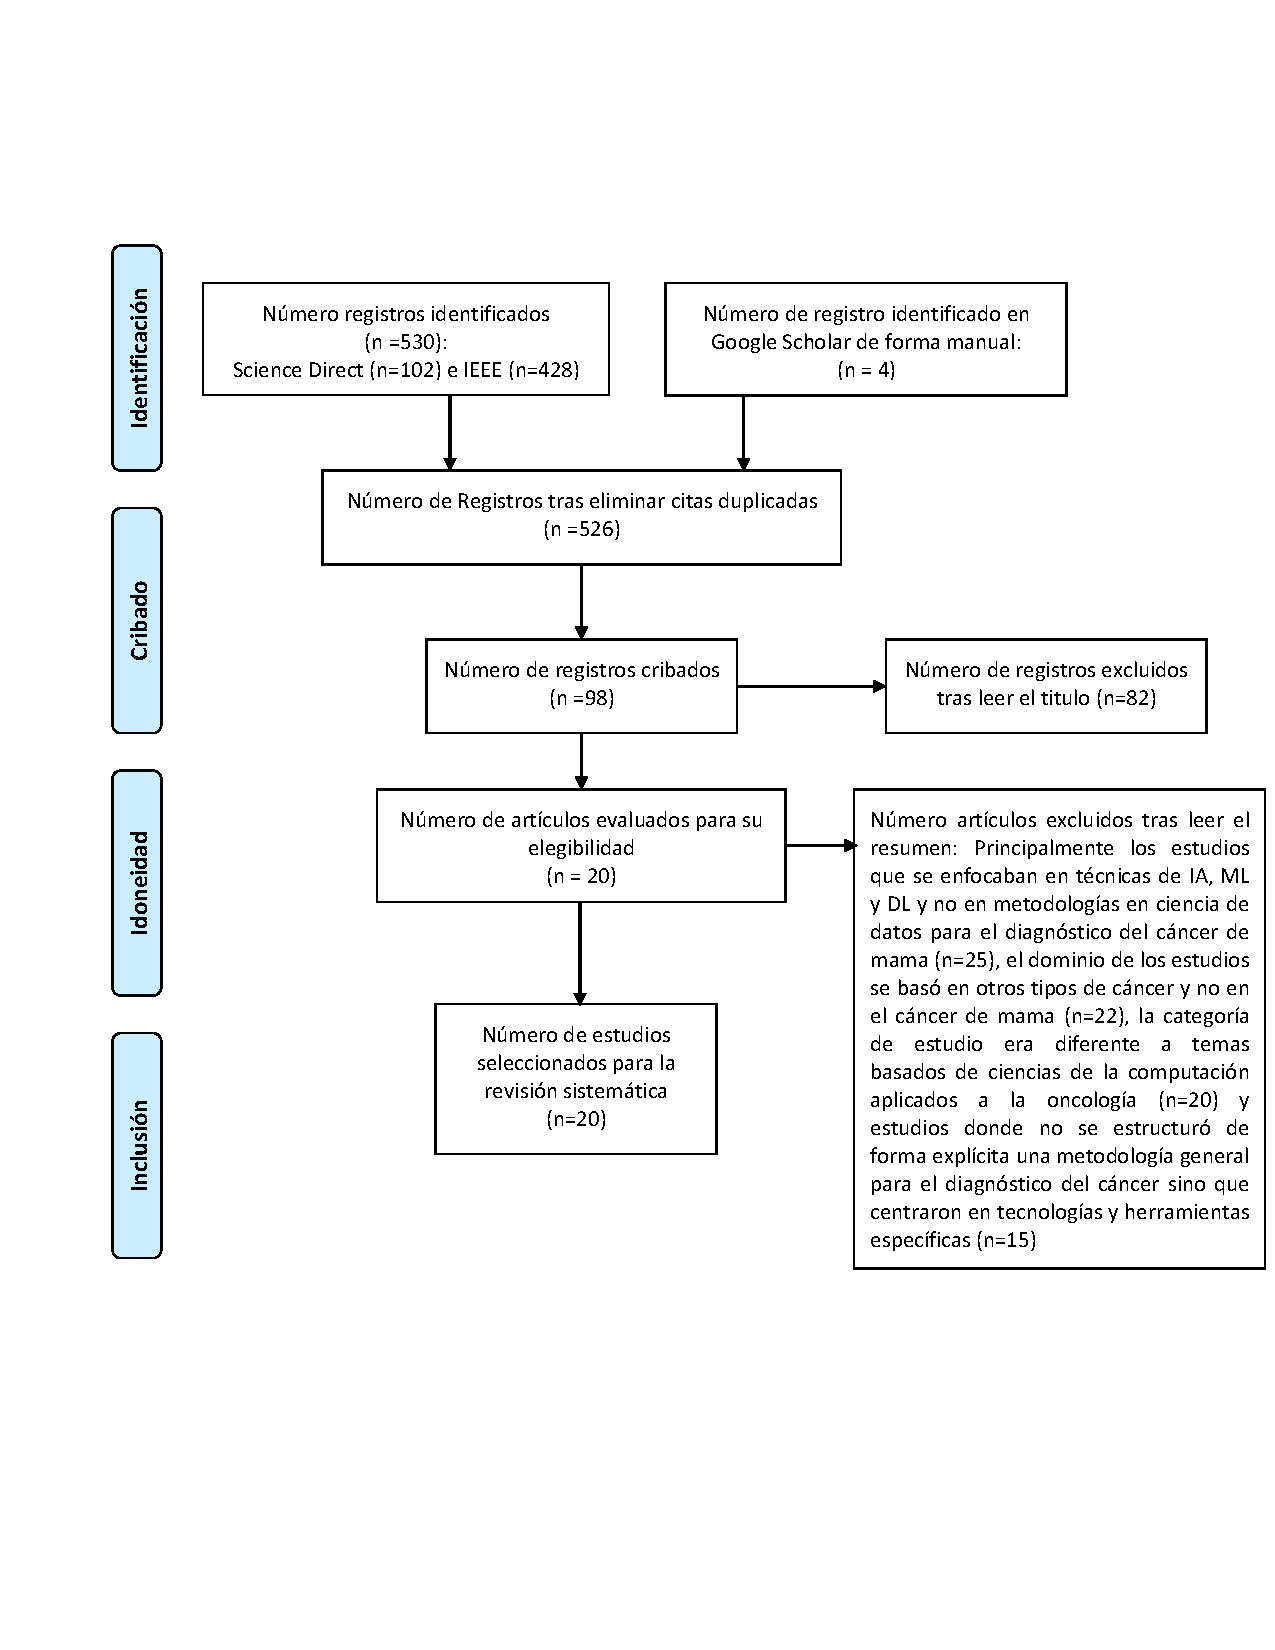
\includegraphics[width=1
	\linewidth]{IMAGENES/PRISMA_DIAGRAM}
	\caption{Diagrama de flujo PRISMA en cuatro niveles }
	\label{Diagrama_Prisma}
\end{figure}

\subsection{Búsqueda inicial}
Las primeras búsquedas se realizaron en abril de 2021 combinando los términos \textit{data science, breast cancer, deep learning, machine Learning, artificial intelligence, cancer Biopsy ,Core needle biopsy, Fine needle aspiration} en las bases de datos de IEEE Access, Nature Reviews Cancer, Elsevier y Science Direct. Posteriormente, para generar una búsqueda mas especifica acerca de metodologías en ciencia de datos aplicadas al diagnostico del cáncer de mama se realizó la combinación de estos términos usando los operadores booleanos \textit{AND} y \textit{OR}. Los resultados obtenidos en la búsqueda arrojaron una cantidad excesiva de literatura basada en técnicas de Inteligencia Artificial, Machine Learning y Deep Learning aplicadas al diagnostico de esta enfermedad sin tener una metodología clara en ciencia de datos aplicada a esta área de la salud, por lo cual dichos resultados fueron poco útiles para la revisión. Sin embargo, las consultas realizadas permitieron tener un visión global de la complejidad del tema de investigación y los diferentes enfoques que pueden generarse a nivel de ciencia de la computación si no se limita la temática al rededor de una metodología.

Debido a que los resultados arrojados por Nature Reviews Cancer y The Lancet estaban enfocados en técnicas y no metodologías, lo cual no aportada información relevante al estudio, se decidió su eliminación de la búsqueda sistemática.  

\subsection{Búsqueda sistemática}
La búsqueda sistemática se realizo en febrero del 2022, en IEEE Access y Science Direct, acotando los resultados de publicaciones realizadas en 2014 hasta la actualidad. La combinación de términos que arrojó mejores resultados en ambos buscadores fue la siguiente:
\textit{(methodology AND Data Science) OR (methodology AND diagnose AND cancer) OR (data science AND methodology AND health AND diagnostics) OR (data science AND methodology AND breast AND cancer)}.

Concretamente, se obtuvieron $530$ resultados de los cuales $428$ fueron encontrados en IEEE Access y $102$ en Science Direct. Antes de realizar la selección de artículos, se definieron los siguientes criterios de inclusión y exclusión. 

\begin{itemize}
	
	\item{\textbf{\textit{Criterios de inclusión}}}
	\begin{itemize}
		\item Tratarse de artículos de investigación, revisión sistemática, libros o manuales. 
		\item Que los estudios realizados estén basadas en metodologías en ciencia de datos  y no en técnicas de Inteligencia Artificial, Machine Learning y Deep Learning.
		\item Que la categoría de estudio este bajo la temática de ciencias de la computación aplicado a la oncología.
		\item Que el dominio determinado este enfocado en el diagnostico del cáncer de mama.
		\item Que los articulo de investigación realizados no dependan de tecnologías ni herramientas específicas.
		\item Que se hayan publicado entre 2014 y 2022, ambos inclusive.
		
	\end{itemize}
	
	\item{\textbf{\textit{Criterios de exclusión}}}
	\begin{itemize}
		\item Se excluyen los estudios que se enfoquen en técnicas de Inteligencia Artificial, Machine Learning y Deep Learning y no en metodologías en ciencia de datos. 
		\item Estudios en donde el dominio se base en otros tipos de cáncer y no en el cáncer de mama.
		\item Estudios donde la categoría sea diferente a temas basados de ciencias de la computación aplicados a la oncología. 
		\item Estudios donde no se evidencie de forma explícita una estrategia general para el diagnóstico del cáncer sino se centren en otros temas, tecnologías y herramientas específicas.
	\end{itemize}
	
\end{itemize}

Según estos criterios, y sólo con la lectura del titulo se consideraron adecuados $98$ artículos. Posteriormente, se realizo la lectura del resumen y a partir de esta lectura, se descartaron $82$ artículos, principalmente los estudios que se enfocaban en técnicas de Inteligencia Artificial, Machine Learning y Deep Learning y no en metodologías en ciencia de datos para el diagnóstico del cáncer de mama ($n=25$), el dominio de los estudios se basó en otros tipos de cáncer y no en el cáncer de mama ($n=22$), la categoría de estudio era diferente a temas basados de ciencias de la computación aplicados a la oncología ($n=20$) y estudios donde no se estructuró de forma explícita una metodología general para el diagnóstico del cáncer sino que centraron en tecnologías y herramientas específicas ($n=15$). Finalmente, $16$ artículos encontrados en IEEE Access y Science Direct cumplieron con los criterios de inclusión y se seleccionaron para llevar a cabo la revisión sistemática. 

\subsection{Búsqueda Manual}
Al realizar una lectura detallada de las $16$ investigaciones encontradas en la búsqueda sistemática, basándonos en sus referencias para comprobar si existía información adicional relacionada con el tema de estudio, se empleo Google Scholar con los términos de búsqueda descritos anteriormente y como resultado se incluyeron $3$ capítulos de libros de ciencias de la computación que abarcaban diferentes metodologías en ciencia de datos y $1$ articulo de investigación encontrado en la revista IJSR\footnote{International Journal of Science and Research } que contenía información relevante para la investigación. 

En definitiva, $20$ investigaciones entre artículos y capítulos de libros publicados entre 2014 y 2022 fueron seleccionados para realizar la revisión sistemática de la aplicación de la ciencia de datos en metodologías para el diagnóstico del cáncer de mama (Figura \ref{Diagrama_Prisma}).
\chapter{Resultados}
\section{Discusión}
Según los resultados obtenidos, se infiere que en la información revisada no existe una metodología en ciencia de datos definida para el diagnóstico del cáncer de mama. En efecto, la mayoría de la literatura científica apunta directamente al uso de técnicas de ML y DL para el diagnóstico o pronostico del cáncer de mama exponiendo el nivel de precisión, cantidad de falsos positivos, gasto computacional y modelos algorítmicos utilizados para determinar el posible padecimiento de esta enfermedad. Y aunque estas investigaciones, brindan información valiosa para mejorar la precisión, sensibilidad y especificidad de las técnicas de ML y DL en el diagnóstico del cáncer, carecen de una metodología clara en donde la idea principal gire entorno de la comprensión del dominio y la toma de decisiones por parte de los oncólogos. En particular, la mayoría de investigaciones llegan a resultados en términos de precisión y exactitud, pero no profundizan en el valor real que el especialista en oncología atribuye a los datos para tomar una decisión y el impacto que dicha decisión tiene en la usabilidad del modelo generado, a sabiendas que el experto a través de su perspicacia medica es quien finalmente evalúa si los resultados obtenidos por los algoritmos son veraces y permiten diagnosticar el cáncer de forma ágil, generando un valor agregado que cumpla con los objetivos de las ciencias de la salud. Por consiguiente, aunque la comunidad de investigación en ciencia de datos este en crecimiento constante, esté explorando nuevos dominios, creando nuevos roles especializados y este realizando un gran esfuerzo de investigación para desarrollar análisis avanzados, mejorar modelos de datos y generar nuevos algoritmos apoyados de los campos de las matemáticas, la estadística y la informática, estas habilidades no son suficientes para la aplicación de la ciencia de datos en proyectos reales \citep{Martinez2021}, puesto que la mayoría de proyectos basados en datos presentan problemas organizativos y socio-técnicos, tales como: una falta de visión y claridad en los objetivos, un énfasis sesgado en cuestiones técnicas y ambigüedad de los roles. Dicho lo anterior, aunque las metodologías seleccionadas en la revisión sistemática no giren en torno al cáncer, proponen etapas que abarcan aspectos relevantes en la organización, a nivel de planteamiento y ejecución de un proyecto en ciencia de datos que tiene como eje el dominio basado en la prevención, el diagnostico y el tratamiento del cáncer de mama. Cabe resaltar que las metodologías CRISP-DM y KDD fueron seleccionadas debido a que comprenden todas las fases básicas que debe cumplir cualquier proyecto que tenga en su contexto el análisis de datos, ademas de que son bastante utilizadas por una cantidad considerable de investigadores, sin embargo aunque sean las metodologías más utilizadas, carecen de lineamientos que profundicen en la organización de los equipos de trabajo para llevar a cabo procesos de gestión que se alienen con el software y las metodologías de desarrollo ágiles. Ademas, autores como \citep{Martinez2021} sugieren que para ofrecer una solución integral para la ejecución exitosa de una metodología en ciencia de datos se deben cubrir estrictamente tres áreas: gestión de proyectos, gestión de equipos y gestión de datos e información. 
Por consiguiente, tras el esfuerzo por integrar los resultados analizados en este trabajo, parece bastante plausible afirmar que no existe una metodología puntual en ciencia de datos que se enfoque en el diagnóstico del cáncer de mama, sin embargo, diversos autores proponen metodologías que permiten la aplicación de esta ciencia en el dominio de las ciencias de la salud, teniendo como eje principal la comprensión de aspectos como: la comunicación constante con los interesados, el uso del enfoque ágil, la definición de roles y funciones, el valor agregado de los datos, la retroalimentación continua y la aceptación del experto en oncología para la posterior toma de decisiones que ayude a reducir de manera eficaz la morbilidad causada por esta enfermedad.

%\section{CONCLUSIÓN}
Con respecto a las metodologías revisadas cabe señalar que no tienen un dominio especifico, por lo tanto queda abierto para los interesados en el análisis de datos la selección de la metodología para un problema determinado. Dicho lo anterior, en la revisión se encontraron metodologías, que aunque abarcan el proceso necesario para el análisis de datos, no generan el valor suficiente para la solución de un problema determinado. Por esta razón, autores como \citep{Martinez2021} consideran que aunque la comunidad de investigación en ciencia de datos está creciendo día a día, esté explorando nuevos dominios, creando nuevos roles especializados y adicional este realizando un gran esfuerzo de investigación para desarrollar análisis avanzados, mejorar modelos y generar nuevos algoritmos apoyados de los campos de las matemáticas, la estadística y la informática, estas habilidades no son suficientes para su aplicación en proyectos reales, puesto que, presentan problemas organizativos y socio-técnicos ,tales como: la falta de visión, objetivos poco claros, un énfasis sesgado en cuestiones técnicas, un bajo nivel de madurez para proyectos ad-hoc y la ambigüedad de los roles. Aunque estos problemas existen en proyectos de ciencia de datos del mundo real, la comunidad no se ha preocupado demasiado por ellos y no se ha escrito lo suficiente sobre las soluciones para abordar estos problemas.

Para comprender mejor, autores como\citep{Schroer2021} consideran que aunque CRISP-DM sigue siendo un estándar por defecto en la minería de datos tiene inconvenientes, ya que la mayoría de los estudios no prevén una fase de implementación. De igual modo, \citep{Martinez2021} consideran que aunque CRISP-DM sigue siendo la metodología más popular para proyectos de análisis, minería de datos y ciencia de datos, no explica cómo deben organizarse equipos de trabajo para llevar a cabo procesos de gestión que se alineen con el software, las metodologías de desarrollo ágiles, y las actividades individuales dentro de cada unas de las etapas que la componen. 

Algo semejante sucede con las metodologías KDD y SEMMA, antecesoras de CRISP-DM. Por el lado de KDD, tenemos que aunque se parte del entendimiento del dominio, su ciclo de vida termina en la visualización e interpretación del conocimiento obtenido sin incluir la retroalimentación por parte del experto; Por lo tanto, aunque se evalué la precisión de los modelos utilizados, esto no es suficiente para determinar si el conocimiento obtenido fue suficiente para tomar una decisión que ayude a solucionar un problema en especifico.   

% PASA uses footnotes, not endnotes. \endnote in this template will behave like \footnote; and \printendnotes will not output anything.
% \printendnotes

\bibliographystyle{unsrt}
\bibliographystyle{apalike}
\newpage

\bibliography{REFERENCIAS/articulos}
%\appendix
%\input{example-appendices}

\end{document}
